 
  \documentclass[final]{beamer} % beamer 3.10: do NOT use option hyperref={pdfpagelabels=false} !

  %\documentclass[final,hyperref={pdfpagelabels=false}]{beamer} % beamer 3.07: get rid of beamer warnings
  \mode<presentation> {  %% check http://www-i6.informatik.rwth-aachen.de/~dreuw/latexbeamerposter.php for examples
    \usetheme{Berlin}    %% you should define your own theme e.g. for big headlines using your own logos 
  }
\setbeamercolor{block body}{bg=white, fg=black}
\setbeamerfont{block title}{size=\Large}
  \usepackage[english]{babel}
  \usepackage[latin1]{inputenc}
  \usepackage{amsmath,amsthm, amssymb, latexsym}
  \usepackage{float}
\usepackage{color}
\usepackage{pgfplots}
\usepackage{anyfontsize}
  %\usepackage{times}\usefonttheme{professionalfonts}  % times is obsolete
  \usefonttheme[onlymath]{serif}
  \boldmath
  \usepackage[orientation=portrait,size=a0,scale=1.2, debug]{beamerposter}                       % e.g. for DIN-A0 poster
  %\usepackage[orientation=portrait,size=a1,scale=1.4,grid,debug]{beamerposter}                  % e.g. for DIN-A1 poster, with optional grid and debug output
  %\usepackage[size=custom,width=200,height=120,scale=2,debug]{beamerposter}                     % e.g. for custom size poster
  %\usepackage[orientation=portrait,size=a0,scale=1.0,printer=rwth-glossy-uv.df]{beamerposter}   % e.g. for DIN-A0 poster with rwth-glossy-uv printer check
  % ...
\definecolor{OliveGreen}{HTML}{eeeeee}

\begin{document}

  \begin{frame}
    \begin{center}

      \textcolor{black}{
      \textbf{\fontsize{110}{40}{\selectfont Panthera: A Study of Caching in 
      Distributed Computing}}}
    \end{center}
    
    \begin{columns}[t]
     \begin{column}{0.32\textwidth}
      \begin{block}{Introduction}
      Distributed computing has seen tremendous growth in the past few years.
In particular, Hadoop, an open source project that allows developers to
write distributed applications, has found extensive use in academia and industry. For example, Yahoo, Facebook, Stanford Computer Science, etc. are all heavily involved with Hadoop development. But, Hadoop does not effectively utilize RAM memory and local storage to better performance. \textbf{This project develops and tests caching mechanisms, called \textbf{Panthera}, to reduce waiting time or latency in Hadoop, } thereby greatly increasing its efficiency and applicability in fields ranging from medical diagnosis to artificial intelligence. 
      \end{block}
      
    \begin{block}{Problem}
	\begin{itemize}
	 \item Develop a caching layer for the Hadoop File System that can cache both data and metadata.
	 \item The solution must not depend on a modified Hadoop version; it should be a "drop-in" addition.
	 \item The layer should reduce file access latency/waiting time significantly in comparison to a vanilla Hadoop installation.
	\end{itemize}

      \end{block}

      \begin{block}{Hypothesis}
       The cache layer designed (called \textbf{Panthera}) will have lower file
       access latency when compared to a standard Hadoop installation. Additionally, it
       will be possible to design \textbf{Panthera} such that the Hadoop source code
       remains unaffected.
      \end{block}
	  
		\begin{block}{Data vs Metadata}
			Data within the Hadoop file system consists of the actual contents of a file.
			Metadata is the information about files and directories, e.g. time a file was created, the list of files in a directory, etc. \textbf{Panthera performs both metadata
			and data caching; both have significantly different technical implications
			and challenges.}
		\end{block}
	
		\begin{block}{Current Hadoop File System Architecture}
			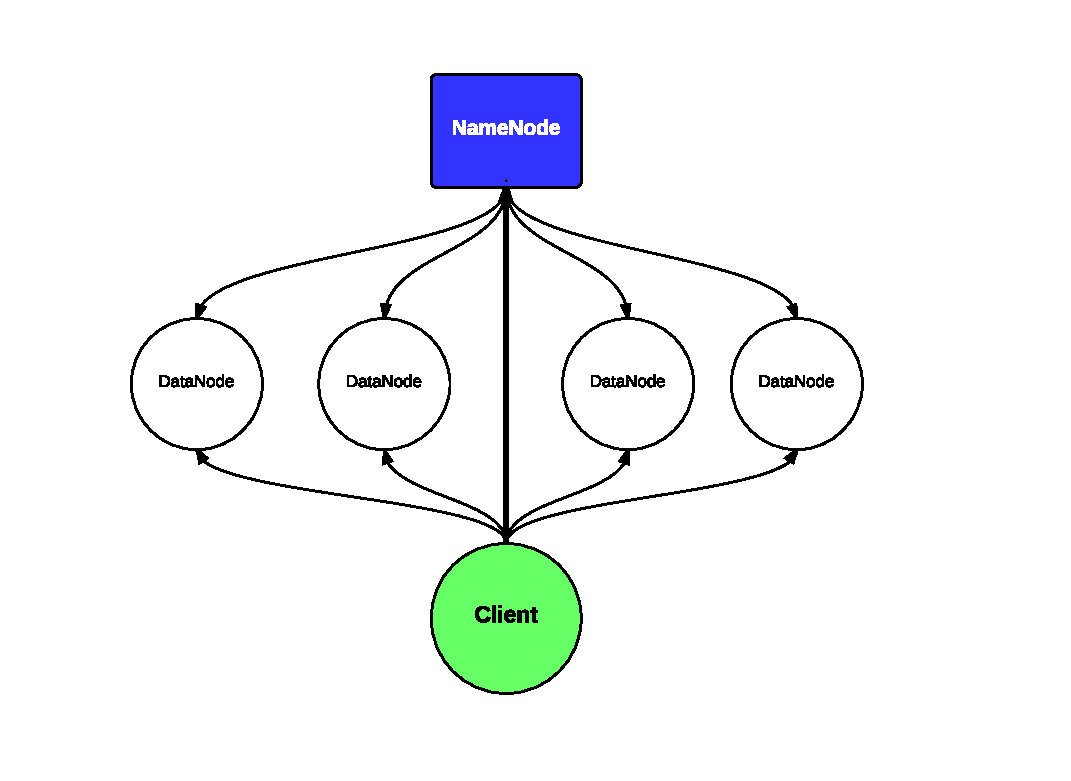
\includegraphics[scale=1]{assets/hadoop_architecture.pdf}
		\end{block}
		
	  \begin{block}{Panthera Architecture}
		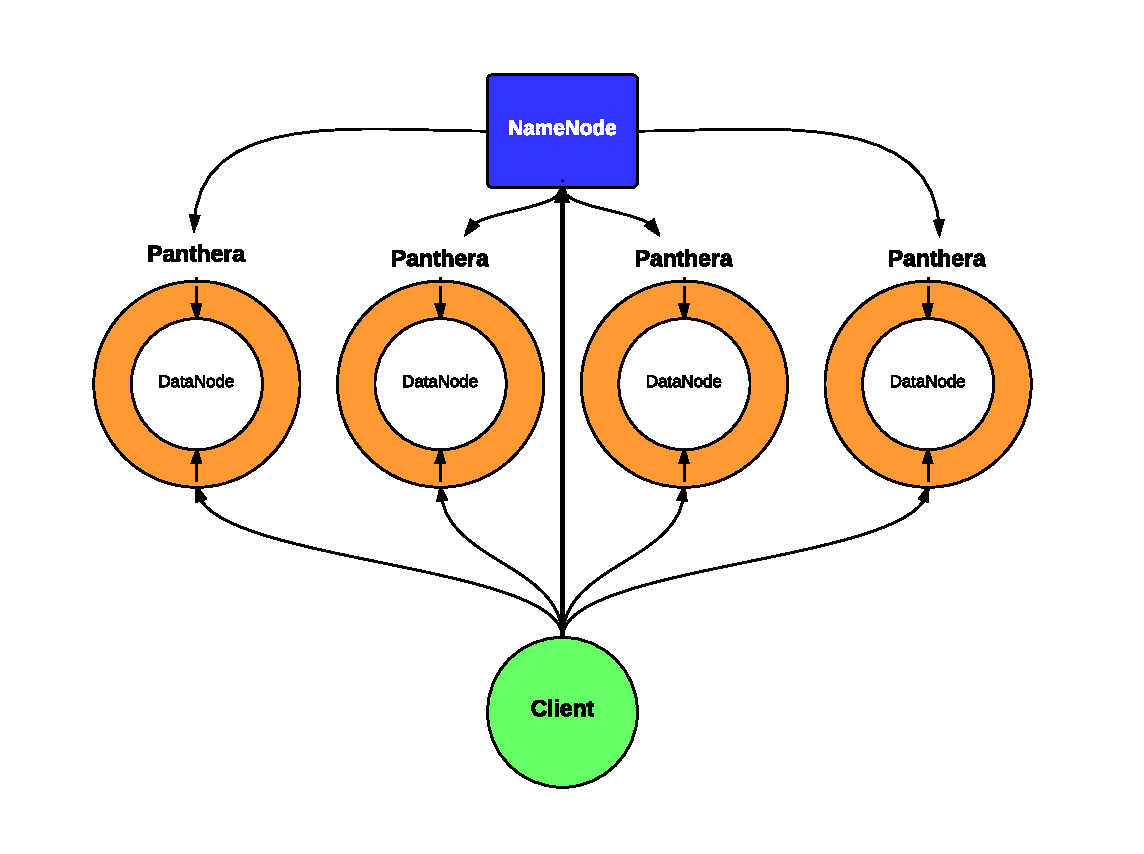
\includegraphics[scale=1]{assets/panthera_architecture_complete.pdf}	  
	  \end{block}
	  
	  \begin{block}{Panthera Metadata Architecture}
	  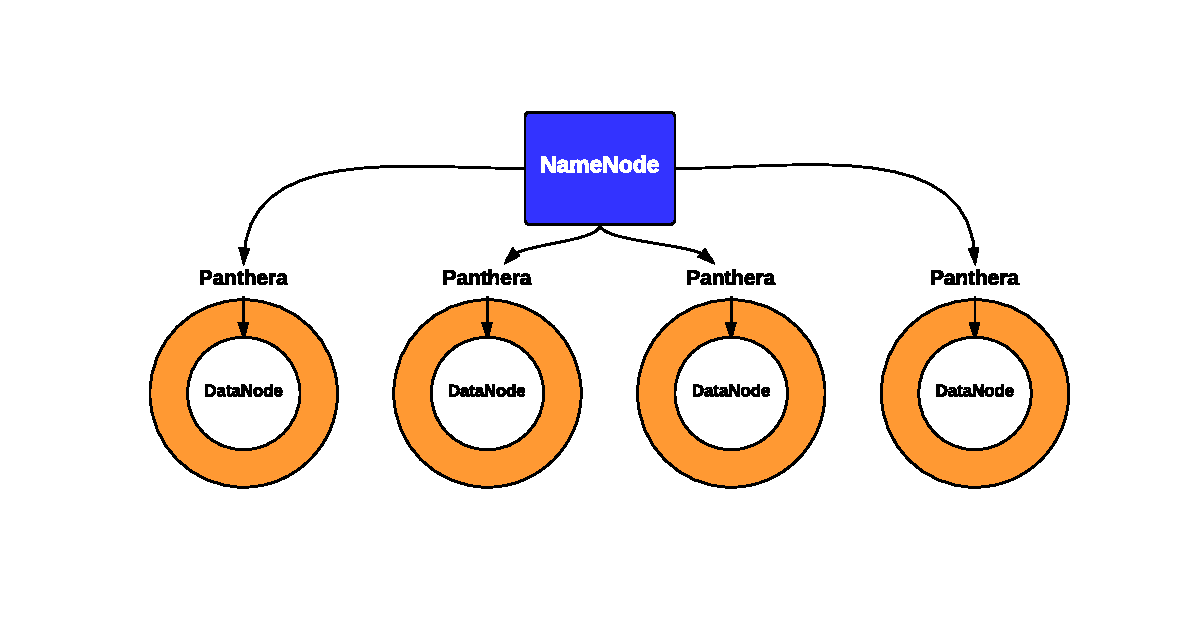
\includegraphics[scale=1]{assets/panthera_metadata.pdf}
      \end{block}
      
      \begin{block}{Panthera Data Architecture}
      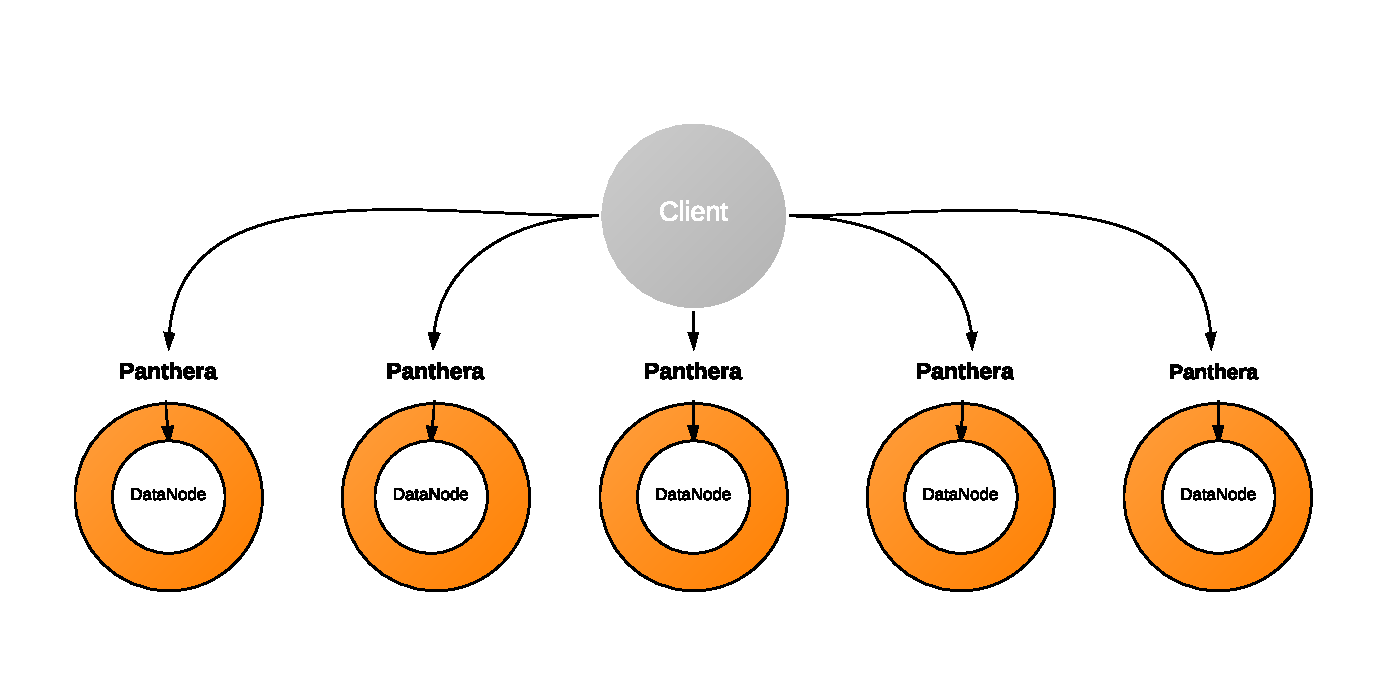
\includegraphics[scale=1]{assets/panthera_architecture.pdf}
      \end{block}

     \end{column}
     %##########################################################################################################

    \begin{column}{0.32\textwidth}

	    
	\begin{block}{Panthera - Implementation}
	\begin{itemize}
		\item \textbf{Panthera is implemented on Google's Go programming language}. The language has excellent concurrency primitives and memory management, which are perfect for
		for software ,such as \textbf{Panthera}, that must run reliably with hundreds of clients.
		\item \textbf{Panthera} implements a large portion of the Hadoop File System protocol, enabling it to "speak" with the DataNode and NameNode.
	\end{itemize}
	\end{block}

	\begin{block}{Testing Methodology - Single Node vs Multinode}
	Testing procedures were conducted on both \textbf{single node} and \textbf{multi-node} setups.\textbf{Single node} testing shows Panthera's performance without regard to network latency, whereas \textbf{multinode} testing incorporates network factors.
	\end{block}
	
	\begin{block}{Testing Methodology - Procedure}
	\begin{itemize}
		\item \textbf{Metadata}: Repeatedly request directory listing for a directory with 100 files in it.
		\item \textbf{Data}: Repeatedly request file contents for a 1MB large file.
	\end{itemize}
	\end{block}

	\begin{block}{Results}
		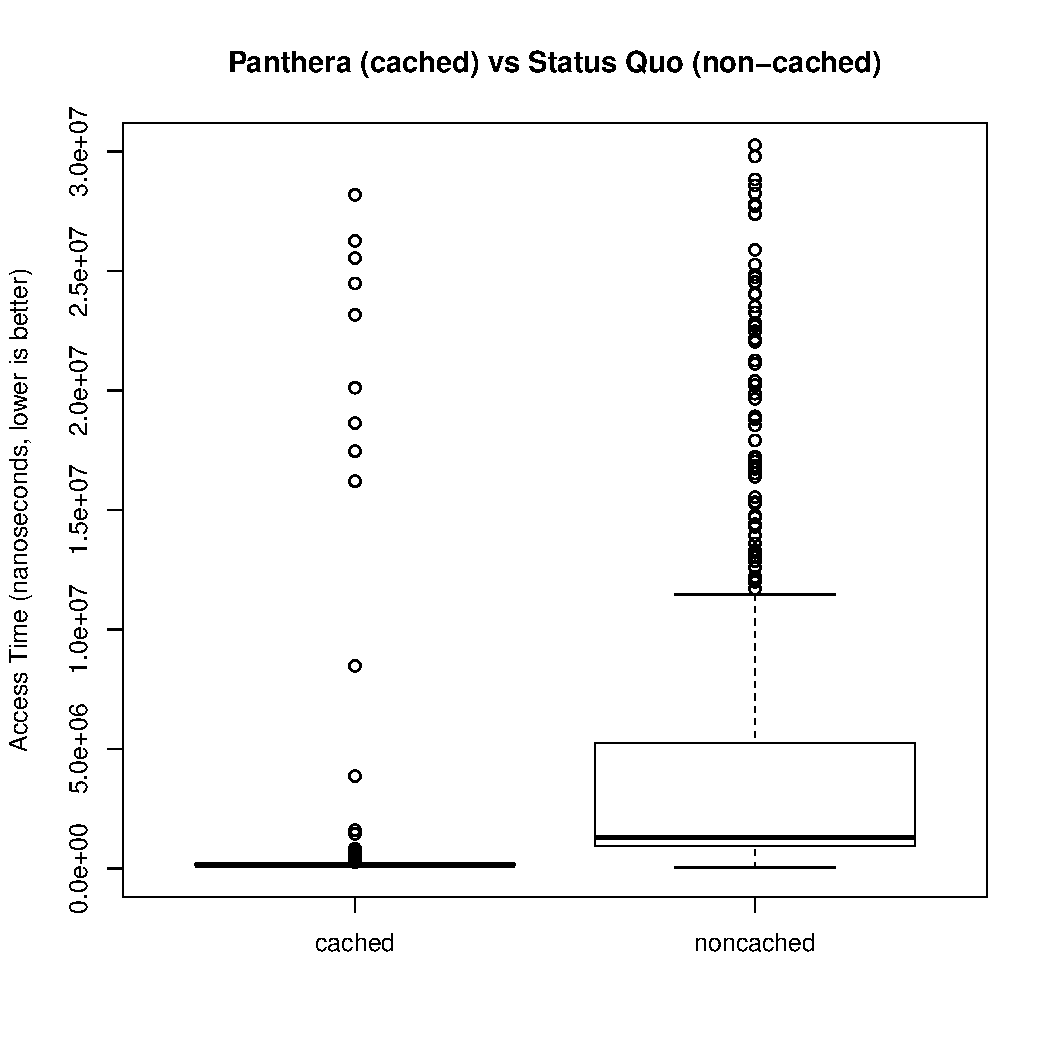
\includegraphics[scale=1.2]{assets/box-plot-data.pdf}
		\vspace{1em}
		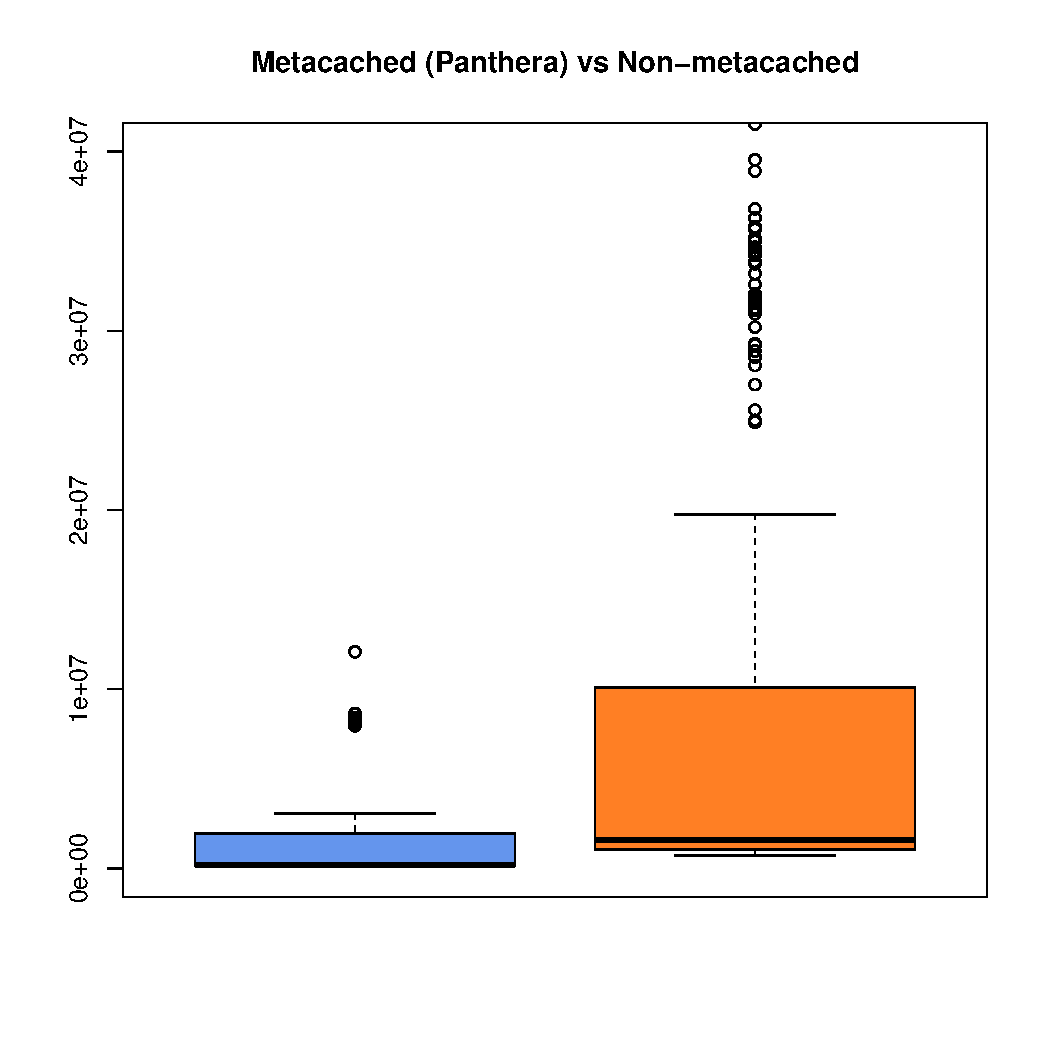
\includegraphics[scale=1.2]{assets/box-plot-metadata.pdf}
		\vspace{1em}
		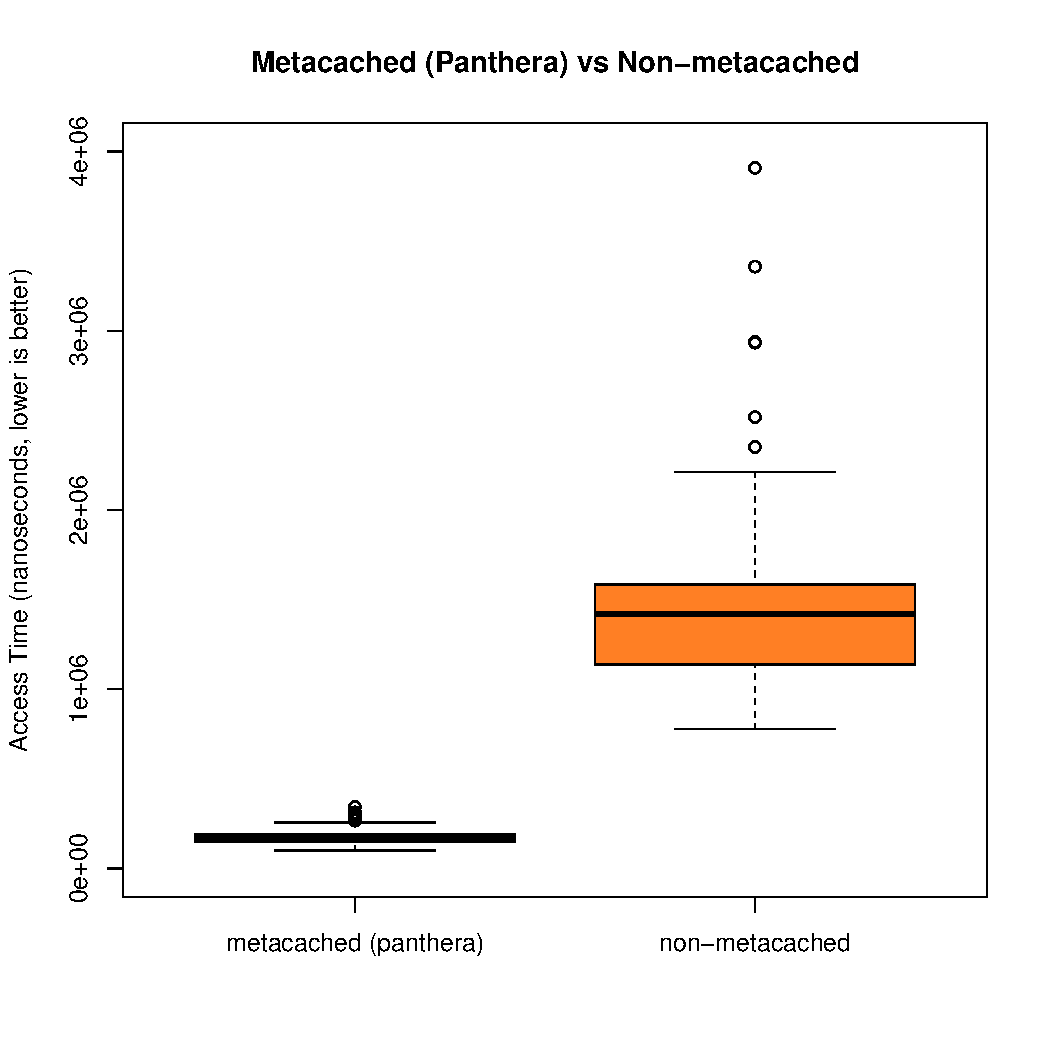
\includegraphics[scale=1.2]{assets/box-plot-meta-multinode.pdf}
	\end{block}

	  
      \end{column}
      %##########################################################
      
      
      \begin{column}{0.32\textwidth}
      
	  \begin{block}{Latency Types}
		%discuss the types of latency and make the comparison
		%between hard disk latency and regular lateny
		In the Hadoop File System Architecture, there are several types of latency involved:
		\begin{itemize}
		\item \textbf{Network latency: } Information shared between client and server (e.g. between a DataNode and a client) has an attached waiting time. With \textbf{Panthera}, this latency is eliminated since the data is cached on the client.
		\item \textbf{Hard drive latency: } Reading from the hard drive has very significant latency. Hadoop generally reads from the hard drive when accessing files.
		\item \textbf{Memory latency: } Reading from RAM memory has an extremely small
		waiting time associated with it. \textbf{Memory waiting time is less than 1/1000th hard drive waiting time. Panthera converts hard drive latency to memory latency, thereby greatly reducing file access time.}
		\end{itemize}
	  \end{block}
	  
    \begin{block}{Statistics}
    \begin{itemize}
    		\item \textbf{Data (single node, noncached)}
    		\begin{itemize}
    			\item Mean: 12548998 nanoseconds
    			%\item Median: 1292182 nanoseconds
    		\end{itemize}
    		\item \textbf{Data (single node, cached/Panthera)}
    		\begin{itemize}
    			\item Mean: 511185.3 nanoseconds
    			%\item Median: 149004 nanoseconds
    		\end{itemize}
    		\item \textbf{Noncached/Panthera}: \textbf{95.9\% improvement in latency with Panthera}, waiting time of noncached is 24.5 times higher than that of Panthera.
    		
    		\item \textbf{Metadata (single node, noncached)}
    		\begin{itemize}
    			\item Mean: 8445265 nanoseconds
    			%\item Median: 1563000 nanoseconds
    		\end{itemize}
    		
    		\item \textbf{Metadata (single node, cached)}
    		\begin{itemize}
    			\item Mean: 1055012 nanoseconds
    			%\item Median: 179500 nanoseconds
    		\end{itemize}
    		
    		\item \textbf{Metadata (multinode, noncached)}
		\begin{itemize}
			\item Mean: 1638184 nanoseconds    		
    		\end{itemize}
    		
    		\item \textbf{Metadata (multinode, Panthera cached)}
    		\begin{itemize}
			\item Mean: 176868.7 nanoseconds    		
    		\end{itemize}
    		
    		\item \textbf{Metadata - noncached/Panthera: } \textbf{90.3\% improvement with the Panthera metadata cache}. Panthera (developed during this project) decreases waiting time by a factor of 8.
    		
	\end{itemize}    	    
    \end{block}
    
    	\begin{block}{Conclusion}
	The results validate the hypothesis presented. Panthera was successfully developed as a "drop-in" solution and it was able to reduce file access latency in comparison to a standard Hadoop installation. In particular, \textbf{the Panthera data cache led to a 95.9\% or 9 fold decrease in waiting time} and the \textbf{the Panthera metadata cache also gave a 90.3\% or 8 fold decrease in latency}. Additionally, the \textbf{the cache developed during this project had a far lower standard deviation for access times and fewer outliers}. For large scale systems such as those in use at major companies and universities, such a drastic decrease in latency can have incredible effects on the efficiency of distributed computing systems.
	
	\end{block}
	
	\begin{block}{Applications}
	Hadoop has diverse applications and since Panthera was created as a "drop-in" solution, the \textbf{applications span an extremely wide range of disciplines}.
	\begin{itemize}
		\item Bioinformatics (e.g. CrossBow from Johns Hopkins University)
		\item Numerical/scientific computing 
		\item Image processing
		\item Artificial Intelligence/Machine Learning (e.g. Apache Mahout)
		\item Market Research (e.g. Target)
	\end{itemize}
	\end{block}
	
	\begin{block}{Future Work}
	\begin{itemize}
		\item \textbf{All code related to this project will be open sourced} to further development in distributed computing.
		\item Currently working on testing a \textbf{bioinformatics toolkit with Panthera}; initial results are very promising and show significant reduction in total running time.
		\item Smart scheduling using Panthera; arranges tasks so that the cache is used most efficiently.
		
	\end{itemize}
	\end{block}
      \end{column}
    \end{columns}
  \end{frame}
    
  \end{document}